%%
%% This is file `sample-sigconf.tex',
%% generated with the docstrip utility.
%%
%% The original source files were:
%%
%% samples.dtx  (with options: `sigconf')
%% 
%% IMPORTANT NOTICE:
%% 
%% For the copyright see the source file.
%% 
%% Any modified versions of this file must be renamed
%% with new filenames distinct from sample-sigconf.tex.
%% 
%% For distribution of the original source see the terms
%% for copying and modification in the file samples.dtx.
%% 
%% This generated file may be distributed as long as the
%% original source files, as listed above, are part of the
%% same distribution. (The sources need not necessarily be
%% in the same archive or directory.)
%%
%% The first command in your LaTeX source must be the \documentclass command.
\documentclass[sigconf]{acmart}

%%
%% \BibTeX command to typeset BibTeX logo in the docs
\AtBeginDocument{%
  \providecommand\BibTeX{{%
    \normalfont B\kern-0.5em{\scshape i\kern-0.25em b}\kern-0.8em\TeX}}}

%% Rights management information.  This information is sent to you
%% when you complete the rights form.  These commands have SAMPLE
%% values in them; it is your responsibility as an author to replace
%% the commands and values with those provided to you when you
%% complete the rights form.
%%\setcopyright{na}
\copyrightyear{2020}
\acmYear{2020}
\acmDOI{na}

%% These commands are for a PROCEEDINGS abstract or paper.
\acmConference[CSML1020]{Machine Learning at Scale}{York University School of Continuing Studies}
%% \acmBooktitle{Project}
%% \acmPrice{free}
%% \acmISBN{978-1-4503-XXXX-X/18/06}


%%
%% Submission ID.
%% Use this when submitting an article to a sponsored event. You'll
%% receive a unique submission ID from the organizers
%% of the event, and this ID should be used as the parameter to this command.
%%\acmSubmissionID{123-A56-BU3}

%%
%% The majority of ACM publications use numbered citations and
%% references.  The command \citestyle{authoryear} switches to the
%% "author year" style.
%%
%% If you are preparing content for an event
%% sponsored by ACM SIGGRAPH, you must use the "author year" style of
%% citations and references.
%% Uncommenting
%% the next command will enable that style.
%%\citestyle{acmauthoryear}

%%
%% end of the preamble, start of the body of the document source.
\begin{document}

%%
%% The "title" command has an optional parameter,
%% allowing the author to define a "short title" to be used in page headers.
\title{Training Neural Networks to Classify Bird Calls}

%%
%% The "author" command and its associated commands are used to define
%% the authors and their affiliations.
%% Of note is the shared affiliation of the first two authors, and the
%% "authornote" and "authornotemark" commands
%% used to denote shared contribution to the research.
\author{Pete Gray}
\authornote{Pete prepared this report, working individually, for the final project in CSML1020 Machine Learning at Scale.}
\email{ptgray@gmail.com}
\email{ptgray@my.yorku.ca}
\email{217653247}
\affiliation{%
  \institution{CSML1020 - Machine Learning at Scale - York University School of Continuing Studies}
  \streetaddress{4700 Keele St}
  \city{Toronto}
  \state{Ontario}
  \country{Canada}
  \postcode{M3J 1P3}
}

%%
%% By default, the full list of authors will be used in the page
%% headers. Often, this list is too long, and will overlap
%% other information printed in the page headers. This command allows
%% the author to define a more concise list
%% of authors' names for this purpose.
\renewcommand{\shortauthors}{Gray}

%%
%% The abstract is a short summary of the work to be presented in the
%% article.
\begin{abstract}
  Neural Networks can be trained to recognize bird calls. In this project,
  a number of approaches to this task are taken. Accurate classification of
  numerous species of birds requires computationally intense training of
  deep algorithms. Approaches to achieving computational 
  intensity are explored in this project as well.
\end{abstract}

%%
%% The code below is generated by the tool at http://dl.acm.org/ccs.cfm.
%% Please copy and paste the code instead of the example below.
%%
\begin{CCSXML}
<ccs2012>
<concept>
<concept_id>10010147.10010257</concept_id>
<concept_desc>Computing methodologies~Machine learning</concept_desc>
<concept_significance>500</concept_significance>
</concept>
<concept>
<concept_id>10010147.10010257.10010293</concept_id>
<concept_desc>Computing methodologies~Machine learning approaches</concept_desc>
<concept_significance>500</concept_significance>
</concept>
<concept>
<concept_id>10010147.10010257.10010293.10010294</concept_id>
<concept_desc>Computing methodologies~Neural networks</concept_desc>
<concept_significance>500</concept_significance>
</concept>
<concept>
<concept_id>10010147.10010257.10010321</concept_id>
<concept_desc>Computing methodologies~Machine learning algorithms</concept_desc>
<concept_significance>500</concept_significance>
</concept>
<concept>
<concept_id>10010147</concept_id>
<concept_desc>Computing methodologies</concept_desc>
<concept_significance>500</concept_significance>
</concept>
<concept>
<concept_id>10010147.10010178</concept_id>
<concept_desc>Computing methodologies~Artificial intelligence</concept_desc>
<concept_significance>300</concept_significance>
</concept>
<concept>
<concept_id>10010147.10010178.10010216</concept_id>
<concept_desc>Computing methodologies~Philosophical/theoretical foundations of artificial intelligence</concept_desc>
<concept_significance>300</concept_significance>
</concept>
<concept>
<concept_id>10010147.10010178.10010216.10010217</concept_id>
<concept_desc>Computing methodologies~Cognitive science</concept_desc>
<concept_significance>100</concept_significance>
</concept>
</ccs2012>
\end{CCSXML}


\ccsdesc[500]{Computing methodologies~Machine learning}
\ccsdesc[500]{Computing methodologies~Machine learning approaches}
\ccsdesc[500]{Computing methodologies~Neural networks}
\ccsdesc[500]{Computing methodologies~Machine learning algorithms}
\ccsdesc[500]{Computing methodologies}
\ccsdesc[300]{Computing methodologies~Artificial intelligence}
\ccsdesc[300]{Computing methodologies~Philosophical/theoretical foundations of artificial intelligence}
\ccsdesc[100]{Computing methodologies~Cognitive science}


%%
%% Keywords. The author(s) should pick words that accurately describe
%% the work being presented. Separate the keywords with commas.
\keywords{machine learning, convolutional neural networks, training at scale, feature extraction, audio classification}

%% A "teaser" image appears between the author and affiliation
%% information and the body of the document, and typically spans the
%% page.
\begin{teaserfigure}
  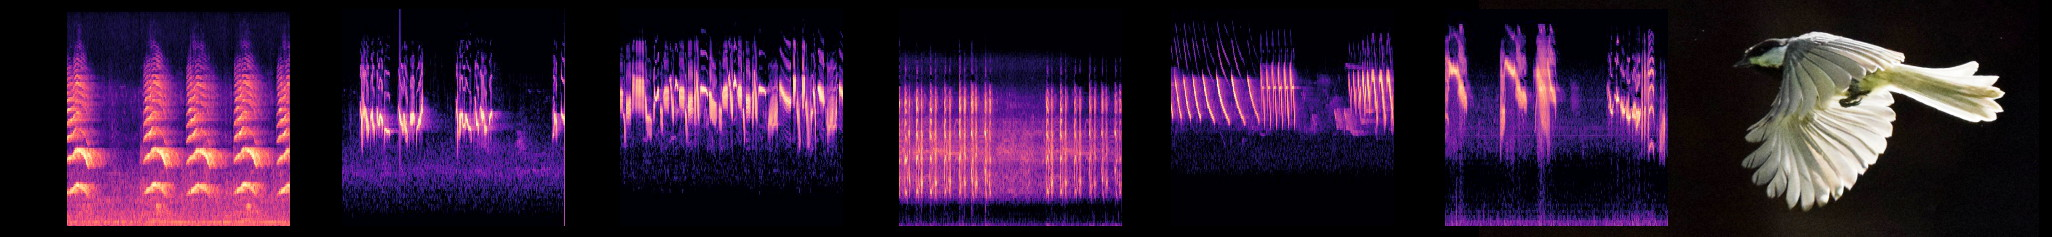
\includegraphics[width=\textwidth]{spectrograms-and-bird}
  \caption{An assortment of spectrograms and a Bird. Photo by Pete Gray}
  \Description{A selection of spectrograms that were derived from the data
used in this project, plus a picture the author took of a bird some years back.}
  \label{fig:teaser}
\end{teaserfigure}

%%
%% This command processes the author and affiliation and title
%% information and builds the first part of the formatted document.
\maketitle

\section{Introduction}
There are a number of commercially available apps that can 
recognize bird song in the field. Training a neural network to 
recognize audio signals is a common task in the field of
machine learning. Data from a 2013 Kaggle Competiton  \cite{Kaggle13} are
used in this project, however the machine learning techniques
used here are perhaps more modern, but certainly quite different.

Cloud-based GPUs are used
to train models that perform accurate classification for the full
range of bird species represented in the data. This cloud-based
training is compared thoughtfully, if not accurately, to similar
training on local computers.

\section{Overview}
Several approaches to audio classification are explored. Two approaches
are explored in depth, with one of those approaches being fleshed out
into a deep exploration of hyperparameter tuning, data augmentation, and
achieving high model performance by leveraging the processing power of
cloud-based computing platforms.

Because this is a project for an academic course, and because the 
definition of the assignment strongly suggests that the journey of
exploration is more important than the quantifiable utility of the results,
an unusually disproportionate amount of time and thought will be put
into abstract intuitions that would fall into the "put yourself in the math's
shoes" category.

%%\url{https://www.acm.org/publications/proceedings-template}.

\subsection{Commercial Implementations}

The use of trained neural networks to identify bird calls is common. A
number of companies and organziations have produced apps that allow
a user to sample audio in the field and perform inference on that audio
in order to identify the species of birds that are audible in the sample.

\begin{itemize}
\item Merlin Bird ID by Cornell Lab  \cite{Merlin20}
\item Song Sleuth \cite{songsleuth20}
\item Chirp-O-Matic \cite{chirp20}
\end{itemize}

One possible commercial venue for the results of this project would be
to produce a simple bird recognition tool that can be embedded on a web
page. Rather than pay to install an app, users could visit the page, be
exposed to an advertisment, and have their local bird species identified 
free of charge. Should this product be developed, it will be called Cheapcheep.

\subsection{Interaction with Human Learning}

One insight into machine learning that these classification tools provide is an illustration of
the power of labeling data. Humans learn to recognize bird calls by hearing them
in the field. Without knowledge of which bird they are hearing, the ability to
identify the species by name will not develop. Traditionally, humans have relied on 
other humans to tell them what type of bird they are hearing - this becomes a "label"
which can be used to infer the species of a bird in the future. Bird call recognition
apps can perform this data labeling function, helping humans become instant 
experts in bird calls, without having to pick the brains of knowledgable humans to get there.

\section{Approaches}

Several approaches were considered. Two approaches were explored. All approaches
had two things in common - a feature extraction phase before model training, and
a deep neural network employed at some point during the process.

\subsection{Spectrograms and a ConvNet}

In this approach, feature selection is performed with Librosa, and
training and inference are done with a convolutional neural net (ConvNet) \cite{xu20} \cite{kaggle18}

\begin{figure}[h]
  \centering
  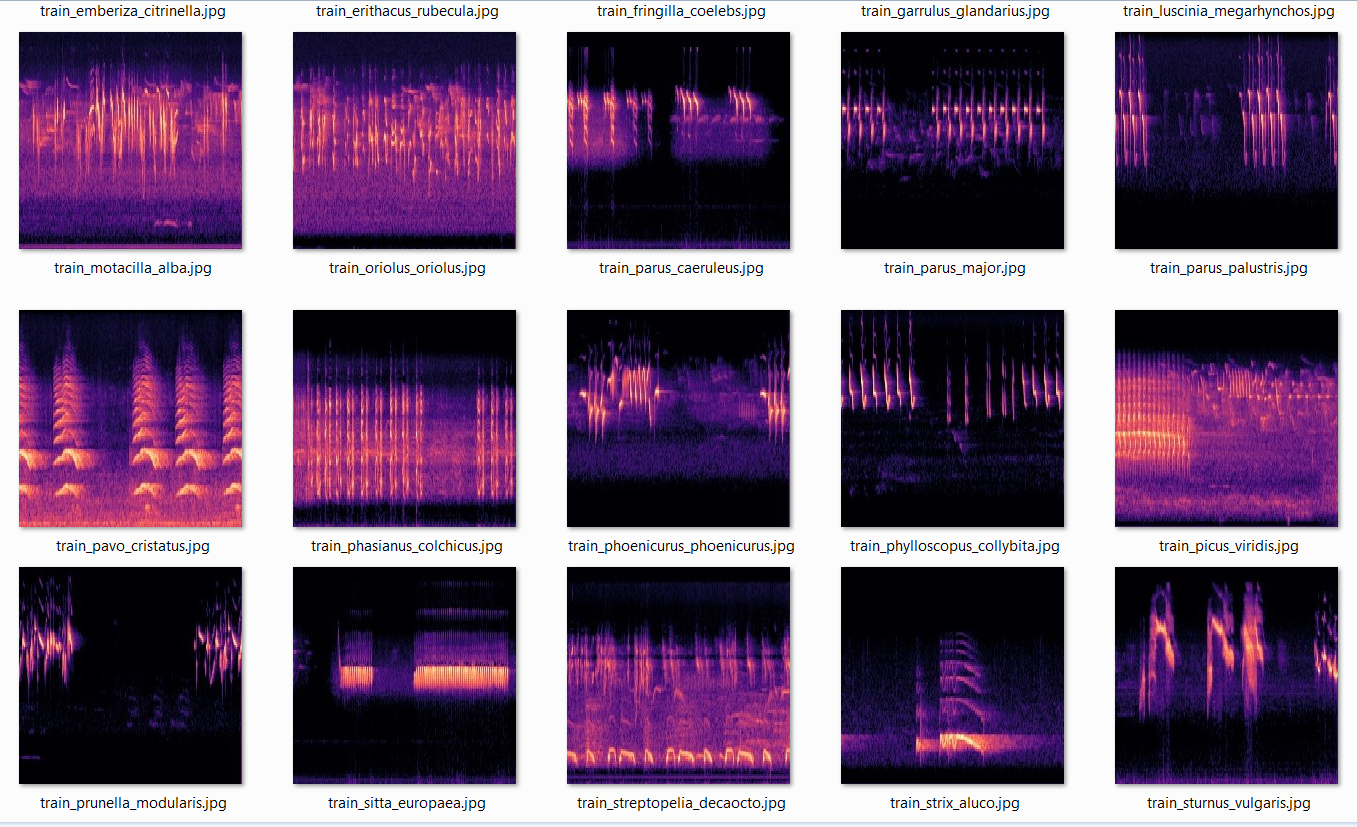
\includegraphics[width=\linewidth]{mfccs_sample_2}
  \caption{A selection of MFCC spectrograms generated from
	audio of bird calls by Librosa.}
  \Description{Spectrograms of bird calls}
\end{figure}

These spectrograms represent the intensity of different sound frequencies
plotted through the duration of the audio samples. It can be clearly seen that
different species of birds produce calls that result in visually distinct spectrograms.
This separation of frequency intensity provides the features, extracted, that
enable the model to train and infer effectively.

Using these spectrograms as inputs,a convolutional neural network can be trained
to perfrom image classification.

For training of models at scale, many samples are taken from the audio files
and converted to spectrograms. Using "sliding windows" as one would with image data,
many samples can be generated up and down the time index of the audio file.

\subsection{Feature Extraction with a Pre-trained VGG-19}

This approach is much more mysterious than the first, and serves best
as a technological curiousity and a point of reference in discussions about
explainability.

A VGG-19 model with pre-trained ImageNet weights is used to extract
features from the raw audio. \cite{mahmood20} To conform to the VGG-19's
input shape, a 224x244 array is created, with one axis being time, and the
other being the intensity of the audio signal. The output of the model
is flattened, resulting in a long vector with 25,088 elements, most of which
are zeroes.

What this vector represents is anyone's guess. The VGG-19's idea of features.
As the neural network was trained using labeled photographs, one wonders
how it must be interpreting these spectrograms. That it's notions get squished 
down into a linear feature vector makes it even more mysterious.

In this approach, the model that is used for inference is a support vector
classifier. (SVC). It is worth noting that the feature vectors emitted by the
VGG-19 bear a strong resemblance to the feature vectors emitted by 
TF-IDF (term frequency, inverse document frequency). which are often used 
with an SVC in the field of natural
language processing (NLP).

\subsection{Comparison of Approaches}

The main differences between these two approaches fell into 3 areas:

\begin{itemize}
\item Power and ease of implementation
\item Explainability
\item The possibility of playing with models in the cloud
\end{itemize}

\subsection{Power and Ease of Implementation}
The VGG-19 approach was very simple to set into motion. Audio
samples are fed into the neural net for inference, one at a time, so
it takes a while but does not demand exceptional computaional resources.
The training of the SVC happens very quickly and achieves very high
validation accuracy (>80\%) on first running.

Using the spectrograms with the untrained network requires model
configuration just to start training. It is very easy to overwhelm the computational
resources by trying to train with too much data. Most early attemps resulted in
very low validation accuracy (<50\%).

\subsection{Explainability} 

While convolutional neural networks themselves aren't exactly the acme
of explainability, the mystery surrounding the training features emitted by
the pre-trained VGG-19 adds a whole new dimension to that.

It is most interesting that despite its mysterious nature, this approach is
able to yield more accurate results so easily. This speaks to the power of 
neural networks, while highlighting their capacity to be inexplicable.

\subsection{The Possibility of Playing with Models in the Cloud}

While compelling in its power, the approach that uses a VGG-19 for
feature extraction doesn't provide the opportunity to play with deep
models. Without some understanding of the feature vectors it emits,
it seems perplexing to imagine re-training the model for improved
performance.

The approach that uses spectrograms, on the other hand, provides
an opportunity to monkey around with every aspect of raw untrained
neural networks.

This approach is therefore chosen for scaling up and playing with models
in the cloud.

\section{Scaling Up}

The ability to train models to recognize bird calls is limited by the processing
power of ordinary computers. By using cloud-based GPUs, both volume of 
data and number of training cycles can be dramatically increased, allowing
meaningful models to be trained in very short periods of time.

\subsection{Preparing to Scale Up}

Programming for data preparation and model training was prepared on
a small scale offline before implemention in the cloud. The implementation
that was successfully trained and played with in the cloud worked well and
was ready for rapid changes to be made to how it worked.

\subsection{Increasing Training Data}

The offline implementation only considered 15 species of birds. It trained
slowly with 4 spectrogram samples for each. After setting it up on a cloud-based
GPU, it was easily able to train on 10 samples from each of the 35 species in the
dataset.

\subsection{Tuning the Models}

With much more data and the potential for deeper training cycles, hyperparameter
tuning provided a variety of ways to improve the training of the models.

It was also observed, with some delight, that reasonasble training could occur over
a very short time period, allowing the programmer to develop more of a "groove"
in which he can bounce ideas quickly off the code to see what sticks.

\subsection{Batch Size, Step Size and Number of Epochs}

These could be increased in the cloud environment, There seems to be a sweet
spot, where a balance of the three yields the best results over a given training time.

\subsection{Learning Rate, Decay, and Momentum}

With different configurations of batch and step size, adjusting the learning rate
slightly from the default value was found to be helpful. It was also seen to be helpful
to customize the decay rate of the learning rate to harmonize with the base rate and 
the number of epochs.

Momentum values were also tweaked experimentally, and while an effect on 
training was observed, it was difficult to see that effect as being helpful.

\subsection{Different Optimizers}
Models were compiled successfully with two different optimizers - RMSprop and Adam.
Adam generally required a much higher learning rate than RMSprop. SGD (stochastic gradient
descent) was also tried, but results were most of the way back to a dummy classifier.

\section{Comparing Cloud GPU Performance}

Many things are different, between training on the laptop and training in the cloud.
Amount of training data, quantity and arrangement of training cycles, and many
hyperparament settings.


To get a feel for the difference in performance between a laptop and a cloud GPU,
we will isolate and compare a small set of factors:

\begin{itemize}
\item Number of classes
\item Validation accuracy of model
\item Training time
\end{itemize}

The following two figures show a stark contrast. In the first, 15 classes are trained
on a laptop (8-core i5), to 45\% accuracy, in 10 minutes. The second shows a model training to
classify 35 species, on a cloud-based GPU, to 93\% accuracy, in 1 minute. 

\begin{figure}[h]
  \centering
  \includegraphics[width=\linewidth]{nice-laptop}
  \caption{Training on an 8-core i5 laptop, 45\% validation accuracy, 10 minutes.}
  \Description{10 minutes on a laptop, 45\%}
\end{figure}

\begin{figure}[h]
  \centering
  \includegraphics[width=\linewidth]{nice-cloud}
  \caption{Training on Google Cloud GPU, 93\% validation accuracy, 1 minute.}
  \Description{1 minute in the cloud, 93\%}
\end{figure}

The dramatic increase in performance can largely be attributed to the much greater volume of
training data. With smaller training sets, the models being trained on the laptop were topping
out at very low numbers, and further training did not change this.

The quicker processing on the cloud GPU allowed the models to train much more quickly, even
though they were processing much more data. 
Based on this example, accounting for both volume of data processed and time to return
results, the difference appears to be well above two orders of magnitude.
It truly made the difference between training 
inadequate models slowly, and training reasonably competent models quickly.

\section{Gratuitous Whimsical Intuition}

From the "put yourself in the math's shoes" file:

As work on this project unfolded, an interesting parallel became apparent.
The machine learning algorithms have a difficult time learning from raw, unprocessed
sequence data. We therefore do feature extraction before training a model. Machine
learning programmers can make better, easier inferences about how their models 
are training by looking at a graph of training data, rather than the raw sequence of
numbers that appears during training.

This meme was created to distill the parallel into a simple idea:

\begin{figure}[h]
  \centering
  \includegraphics[width=\linewidth]{my-model-me-2}
  \caption{Empathizing with ML models on raw data and feature extraction.}
  \Description{Making graphs is like feature extraction for humans}
\end{figure}

Making graphs is like feature extraction for humans.



\section{Summary}
Two approaches to audio classification with deep learning were explored. One used
MFCC spectrographs as input for a convolutional neural net of the type used for image recognition.
The other approach used flattened output from a pre-trained VGG-19 to extract
features for an SVC to use for classification. The spectrograms and convnet approach
was fleshed out in the cloud, where it was possible to quickly train a variety of models
to above 90\% validation accuracy. 

\section{Future Work}

The models used for classification in one appoach were very similar to the models used for feature extraction
in the other approach. Combining the two into a single neural net that can do the feature
extraction and the classification would be interesting. It would also facilitate the development of 
Cheapcheep by only requiring a single piece of technology to be deployed, that can recognize bird calls
all on its own.







%%
%% The next two lines define the bibliography style to be used, and
%% the bibliography file.
\bibliographystyle{ACM-Reference-Format}
\bibliography{sample-base}

%%
%% If your work has an appendix, this is the place to put it.
\appendix



\end{document}
\endinput
%%
%% End of file `sample-sigconf.tex'.
